\documentclass[9pt,twocolumn,twoside]{styles/osajnl}
\usepackage{fancyvrb}
\journal{i524} 

\title{Lighting Memory-Mapped Database (LMDB)}

\author[1]{Leonard Mwangi}

\affil[1]{School of Informatics and Computing, Bloomington, IN 47408, U.S.A.}

\affil[*]{Corresponding authors: lmwangi@iu.edu}

\dates{paper 2 \today}

\ociscodes{Cloud, I524, LMDB, BDB, B+tree}

% replace this with your url in github/gitlab
\doi{\url{https://github.com/cloudmesh/sp17-i524/tree/master/paper2/S17-IO-3012/report.pdf}}

\begin{abstract}
LMDB is one of the most recent in-memory key-value databases, it has
shown performance not matched by many other key-value databases and a
unique capability to manage and reclaim unused space. We’ll examine
the database, it’s architecture, features and use cases that makes it
ideal for self-contained application in need a local small-footprint
database.
\end{abstract}

\setboolean{displaycopyright}{true}

\begin{document}

\maketitle

\section{Introduction}

Lightning Memory-Mapped Database (LMDB) is a high-performance
transaction non-relational database that stores data in the form of
key-value store \cite{www-keyvalue} while using memory-mapped file
capabilities to increase I/O performance. Designed to solve multiple
layers of configuration and caching issues inherent on Berkeley DB
(DBD) design \cite{www-bdb}, LMDB fixes caching problems with a
single, automatically managed cache which is controlled by the host
operating system \cite{www-lmdb}. The database footprint is small
enough to fit in an L1 cache \cite{www-l-cache} and its designed to
always append data at the end of the database (MDB\_APPEND) thus there
is never a need to overwrite data or do garbage collection. This
design protects the database from corruption in case of a system crash
or need to carry out intensive recovery process.

LMDB is built on combination of multiple technologies dating back to
1960s. Memory-Mapped files or persistent object concept was first
introduced by Multics in mid 1960s as single-level storage (SLS)
\cite{www-multics} which provided distinction between files and
process memory this technology incorporated in LMDB architecture. LMDB
also utilizes B+tree architecture which provides a self-balancing tree
data structure making it easy to search, insert and delete data due to
its sorting algorithm. LMDB specifically utilizes the append-only
B+tree code written by Martin Hedenfalk \cite{www-btreecode} for
OpenBSD ldapd implementation. The architecture is also modeled after
BDB API and perceived as it’s replacement.

\section{Architecture}
The following section provides an overview of LMDB architecture and
the technologies involved.

\subsection{Language}

LMDB is written in C but the API supports multiple programming
languages with C and C++ supported directly while other languages like
Python, Ruby, Erlang amongst others supported using
wrappers\cite{www-lmdbwrap}.

\subsection{B+tree}

The append-only B+tree architecture ensures that that the data is
never overwritten thus every time modification is required, a copy is
made and changes made to the copy which is in turn written to a new
disk space. To reclaim the freed space, LMDB uses a second B+tree
which keeps track of pages that have been freed thus keeping the
database size fairly the same. This is a major architectural advantage
compared to other B+tree based databases.

Figure \ref{fig:false-color} Regular B+tree architecture.

\begin{figure}[htbp]
\centering
\fbox{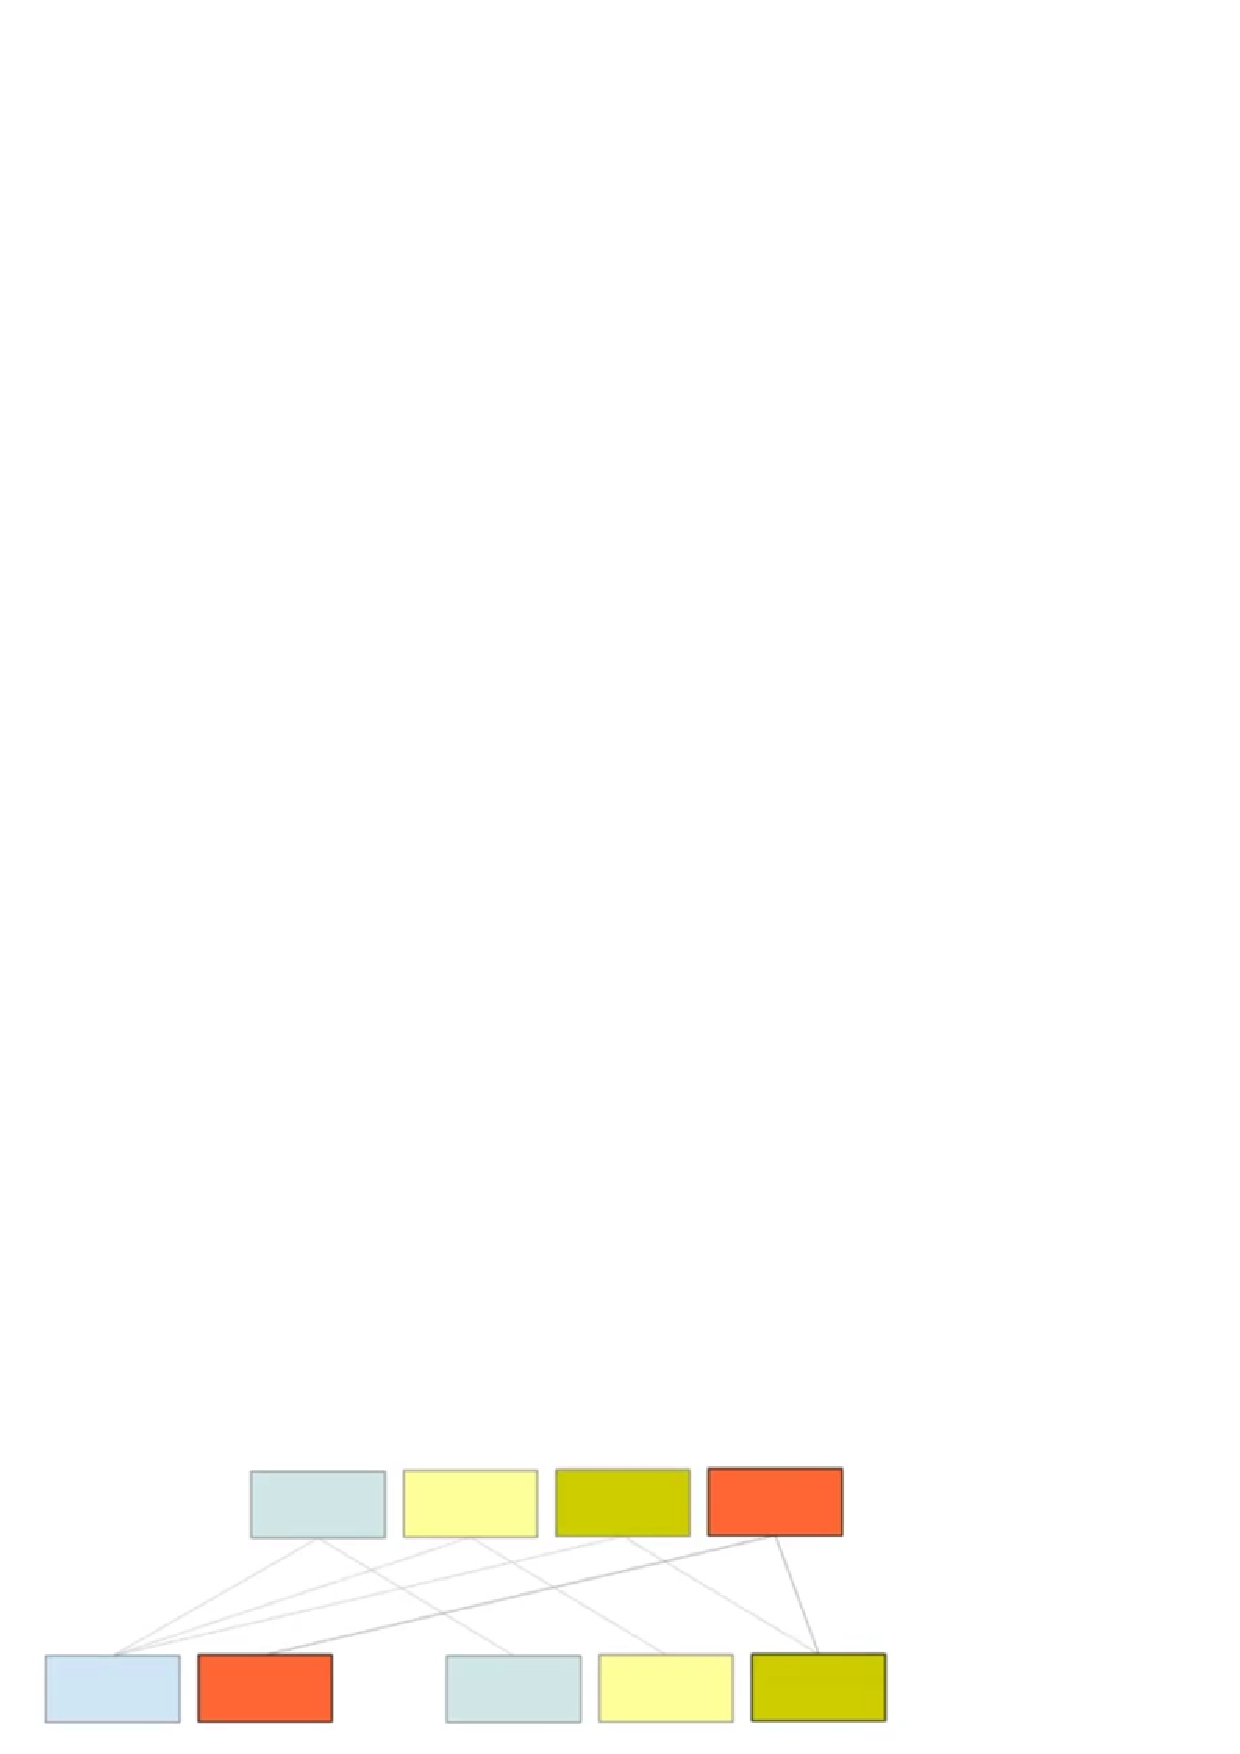
\includegraphics[width=\linewidth]{images/btree1}}
\caption{For every new leaf-node created, a root-node is created}
\label{fig:false-color}
\end{figure}

Figure \ref{fig:false-color} LMDB B+tree architecture.

\begin{figure}[htbp]
\centering
\fbox{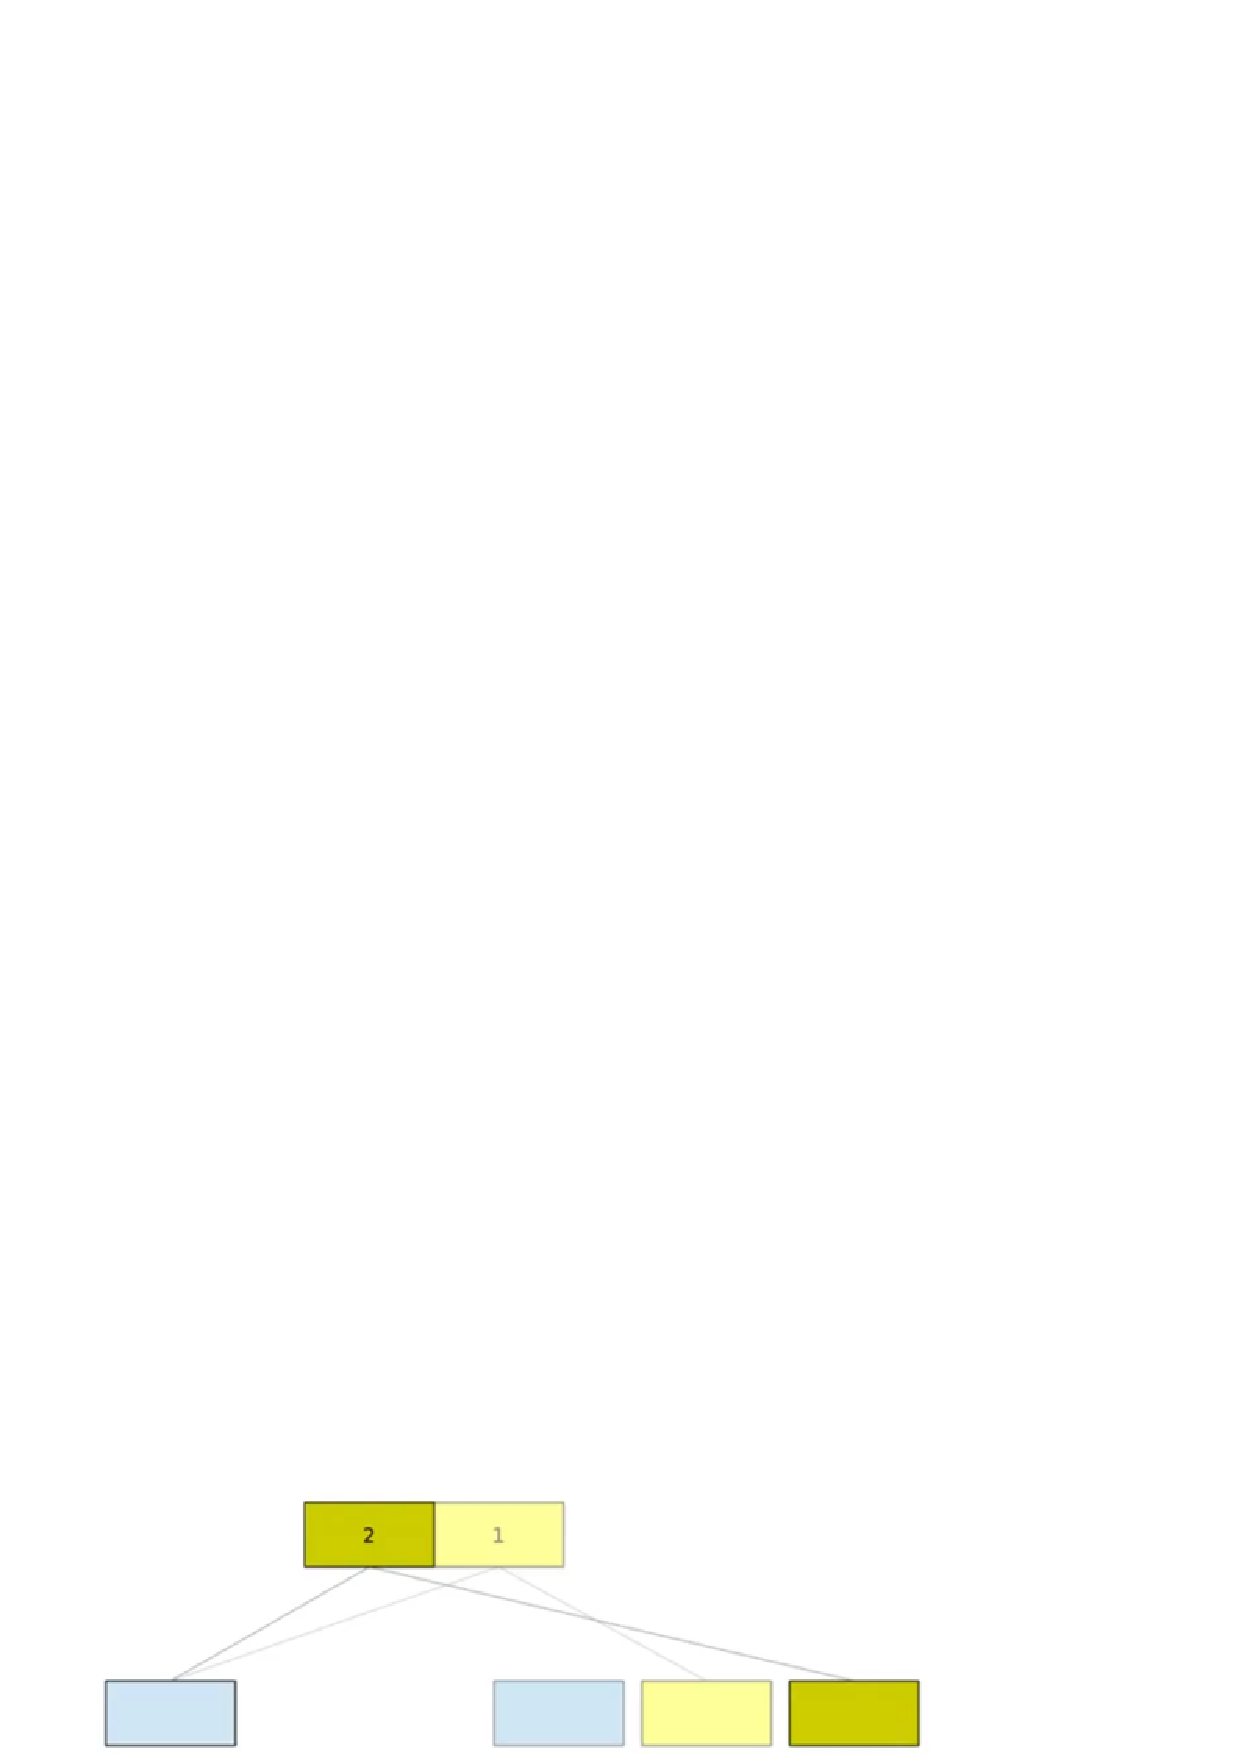
\includegraphics[width=\linewidth]{images/btree2}}
\caption{LMDB uses two root-nodes for valid leaf-nodes as shown in
  diagram above. Unused leaf-nodes do not have root-nodes tied to them
  which signifies unused page that can be reclaimed}
\label{fig:false-color}
\end{figure}

\subsection{Transaction}

The database is architected to support single-writer and many-readers
per transaction \cite{www-lmdbdoc} ensuring no deadlock within the
database. No memory allocation (malloc) or memory-to-memory copies
(memcpy) required by the database thus ensuring that locks do not
occur during

\section{Implementation}

LMDB implementation is supported by both Windows and Unix operating
systems. It is provided in two variants which are automatically
selected during installation. CFFI variant supports PyPy for CPython
version 2.6 or greater and C extensions that support CPython versions
2.5 through 2.7 and version 3.3 and greater. For ease of adoption,
both versions have the same interface. This installation guide will
focus on Python based implementation for both operating systems.  At
the moment 32-bit and 64-bit binaries are provided for Python
2.7. Future binaries are expected to support all versions of Python.

\subsection{Installation}

Installation and configuration process for LMDB.

\begin{figure}[htb]
\begin{quote}
\begin{Verbatim}

#Unix based Systems
pip install lmdb
#or
easyinstall lmdb
#Create and open and environment   
 mdb_env_create() mdb_env_open() #defines the directory path and must
 exist before being used.  #mdb_nosubdir option can be used if no
 directory path needs to be passed. 
#Create transactions after opening the environment
 mdb_env_create() mdb_env_open() #defines the directory path and must
 exist before being used.  #mdb_nosubdir option can be used if no
 directory path needs to be passed. 
#Open database for the transaction
#mdb_dbi_open() #NULL value can be passed if only a single database
    will be used in the environment. 
#mds_create flag must be specified to create a named database. 
#mdb_env_set_maxdbs() defines the maximum number of databases the
    environment will support.
#mdb_get() and #mdb_put() can be used to store a single key/value pairs,
    if more transactions are needed then cursors are required. 
#mdb_txn_commit() is required to commit the data in the environment

\end{Verbatim}
\end{quote}
\caption{LMDB Implementation Code}\label{alg:python}
\end{figure}

\section{Features}

LMDB has the following features that are not in a regular key/value
store databases:

\paragraph {1. Explicit Key Types}
Key comparisons in reverse byte order as well as
native binary integer supported, this goes beyond the regular
key/value string comparisons and memory-to-memory copy.

\paragraph {2. Append Mode}
Useful when bulk loading the data which is already a
sorted format otherwise it would lead to data corruption.

\paragraph{3. Fixed Mapping}
Data can be stored in a fixed memory address where
applications connecting to the database will see all the objects with
the same address.

\paragraph{4. Hot Backups}
Since LMDB uses MVCC, a hot backup can be carried while
the database is live because transactions are self-consisted from
beginning to the end.

\section{Licensing}

LMDB is licensed under OpenLDAP public license, a BSD style
licensing.

\section{Alternatives}

There are several alternatives to LMDB, focusing on key-value
databases, some of the leading alternatives include the following:

\subsection{SQLite3}

One of the alternatives to LMDB, an in-process database designed to be
embedded in the applications rather than having its own server. The
main comparison with LMDB is they are both in-memory databases but
SQLite3 is also a relational database with structured data in form of
tables where is LMDB is not a relational database \cite{www-sqlite}.

\subsection{Oracle Berkeley DB (BDB)}

A key-value database provided in form of software libraries offers an
alternative to LMDB. LMDB is actually molded from DBD thus structure
and architecture is almost the same. BDB is considered to be fast,
flexible, reliable and scalable database and has the ability to access
both key and sequential data. BDB does not require a stand-alone
server and is directly integrated to the application \cite{www-bdb}.

\subsection{Google LevelDB}

LevelDB is an on-disk key-value open source database developed by
google fellows and inspired by BigTable memtable/sstable
architecture. One of the main differences from LMDB is LevelDB
utilizes disk for storage rather than memory which can have negative
impact on performance due to disk seeks \cite{www-riak}. Also, being
an on-disk database, it is susceptible to corruption especially when
there is system crash. LevelDB is licensed under BSD Licensing model
\cite{www-leveldb}.

\subsection{Kyoto Cabinet}

Provided in form of libraries, is an on-disk key-value database with
B+tree and hash tables architecture. Kyoto Cabinet is written in C++
and has APIs for other languages \cite{www-fallabs}. Disk management
has been identified as an issue for Kyoto Cabinet
\cite{www-kyoto}. It’s also licensed under General Public Licensing.

\section{Use Case}

\subsection{NoSQL data Stores}

Due to its small footprint and great performance, LMDB is an ideal
candidate for NoSQL data stores. The data store is widely used for
caching, queue-ing, tasks distribution and pub/sub to enhance
performance. Being an in-memory database, LMDB is a great candidate
for these stores and is currently being used as Redis data store
\cite{www-kyoto}.

\subsection{Mobile Phone database}

In the wake of smart phones, the need for mobile
applications to collect and store data has grown exponentially. Most
of the mobile applications store this data in cloud requiring them to
connect back and forth in order to facility user’s request. Having a
local lightweight self-contained database on the device has become an
attractive solution to enhance user experience with performance and
effectiveness. LMDB fills in this gap due to its small footprint,
performance and ability to reuse storage thus making it a favorable
mobile phone database.

\subsection{Postfix Mail Transfer Agent (MTA) database}

Postfix is an SMTP Server that provides first layer of spambots and
malware defense to the end users. Having the ability to track and keep
history of the scans and identified threats at a fast rate is
paramount for the success of Postfix. Postfix uses LMDB adapter to
provide access to lookup tables and make data available to the
application reliably \cite{www-postfix}.

\section{Conclusion}

Self-managing, small footprint and well performing database is a
critical to many client side applications.  These applications are
better suited when they can offload storage management to the database
application and gain great performance. LMDB has shown these
capabilities by managing how data is written and claiming unused
storage. It’s great performance and small footprint stages it well for
many of the application. In comparison to other databases in its
class, LMDB benchmarks \cite{www-benchmark} shows its capability to be
the leading database on in self-contained application databases. Also,
being available as an OpenLDAP public licensing and having wrappers
for different languages makes it easier to port to already existing
applications.

\section*{Acknowledgements}
This research was done as part of course “I524: Big Data and Open
Source Software Projects” at Indiana University. I thank Professor
Gregor von Laszewski and associate instructors for their support
throughout the course.

% Bibliography

\bibliography{references}
 
\end{document}
